\documentclass[crop=false]{standalone}

\usepackage[subpreambles=false]{standalone}
\usepackage{import}
\usepackage{graphicx}
\usepackage{subcaption}
\usepackage{tikz}

\begin{document}

\begin{figure*}
  \centering
  % \hspace*{-0.08\linewidth}
   \begin{subfigure}[b]{0.2708\textwidth}
  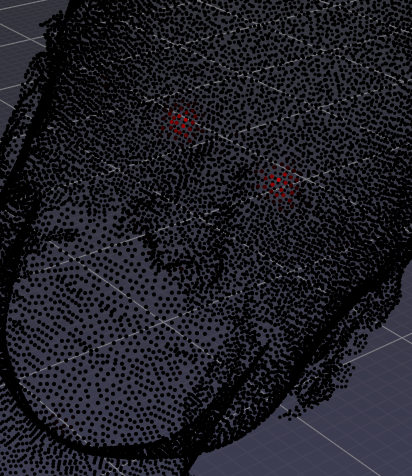
\includegraphics[width=\textwidth]{thesis/methods/import/imgs/a.png}
  \caption{}
  \label{fig:sym_ldmksa}
  \end{subfigure}
  \begin{subfigure}[b]{0.3402\textwidth}
   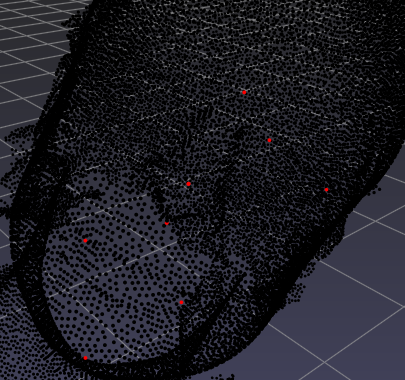
\includegraphics[width=\textwidth]{thesis/methods/import/imgs/b.png}
   \caption{}
   \label{fig:sym_ldmksb}
   \end{subfigure}
   \begin{subfigure}[b]{0.3728\textwidth}
    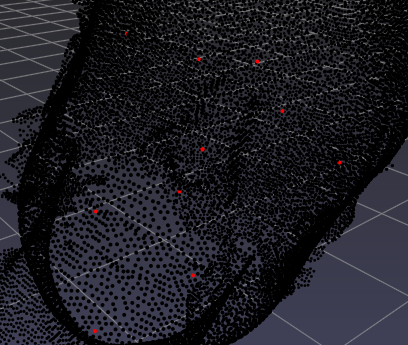
\includegraphics[width=\textwidth]{thesis/methods/import/imgs/c.png}
    \caption{}
    \label{fig:sym_ldmksc}
    \end{subfigure}
  %\vspace*{-0.06\linewidth}
  \caption{\textbf{Symmetrical landmarks issue.}
    \small a) Depiction of the predicted channel for the right endocanthion. Due to the symmetrical landmark problem introduced with HKS features, the network falsely detects both the left endocanthion and right endocanthion in the same channel. b) Before fix: Point landmarks for right endocanthion and right exocanthion identified on the wrong side of the face. c) After fix: Right endocathion and right exocanthion are identified on the correct side of the face.
   }
    
  %\label{fig:sym_ldmks}
\end{figure*}

\end{document}